\section{Step-by-step example: single time-series analysis}
\label{S:ExampleDisp}

This example uses a single synthetic time series data that mimics displacement data measured on a bridge. 

\subsection{Step 1: start a project}

In the \MATLAB{} command window, type \colorbox{light-gray}{\lstinline[basicstyle = \mlttfamily \small, backgroundcolor = \color{light-gray}]!OpenBDLM_main;! }, and type $\dlsh$.
The \lstinline[basicstyle = \mlttfamily \small, backgroundcolor = \color{light-gray}]!OpenBDLM_main! starting menu appears.
The user has to provide an input from the command line each time a \lstinline[basicstyle = \mlttfamily \small, backgroundcolor = \color{light-gray}]!choice >>! appears.
The provided input is validated by typing $\dlsh$.
 \begin{lstlisting}[ frame = single, basicstyle = \mlttfamily \small, caption = {OpenBDLM command line interaction when calling \lstinline!OpenBDLM\_main();!} from \MATLAB{} command line, label = LST:OpenBDLMStartingMenuExample1 ,  float =h!, linewidth=\linewidth, captionpos=b]

------------------------------------------------
     Starting OpenBDLM_V1.0
------------------------------------------------
            Time series analysis using 
            Bayesian Dynamic Linear Models
------------------------------------------------
- Start a new project: 

     *      Enter a configuration filename 
     0   -> Interactive tool 

- Type D to Delete project(s), V for Version control, Q to Quit.

     choice >> 0
  
---------------------------------------
          Starting a new project...
----------------------------------------

- Enter a project name (max 25 characters):
     choice >> DISP
     
- Does this project aim to create synthetic data ? (y/n) 
     choice >> no

     Load data...

- Choose a database

     0   -> Build a new database     	
 
     choice >> 0
\end{lstlisting}

First, choose the interactive tool by typing \colorbox{light-gray}{\lstinline[basicstyle = \mlttfamily \small, backgroundcolor = \color{light-gray}]!0!}.
Secondly, provide a project name (e.i \lstinline[basicstyle = \mlttfamily \small, backgroundcolor = \color{light-gray}]!DISP!).
Then, answer \colorbox{light-gray}{\lstinline[basicstyle = \mlttfamily \small, backgroundcolor = \color{light-gray}]!no!} to indicate that you are not concerned with creating synthetic data.
The next step is to type \colorbox{light-gray}{\lstinline[basicstyle = \mlttfamily \small, backgroundcolor = \color{light-gray}]!0!} to indicate that you aim to load new data.

\subsection{Step 2: load the data}

At this stage, a graphical user interface \footnote{Douglas M. Schwarz, 2007, uipickfiles \url{https://www.mathworks.com/matlabcentral/fileexchange/10867-uipickfiles-uigetfile-on-steroids}} should appear on screen. 
Browse the ``data/csv'' folder to select the csv file named \lstinline[basicstyle = \mlttfamily \small, backgroundcolor = \color{light-gray}]!DISP_DISP.csv!.
Then, click on the Add button, and then the Done button, as highlighted in Figure~\ref{fig:DataLoadingUIPickFileExample1}.
You will notice that some basic information regarding the loaded time-series, such as the time series index, the reference name and the number of data points are now displayed in the \MATLAB{} command window, as depicted in Listing~\ref{LST:OpenBDLMDataAvailabilityExample1}.
At this time, three \MATLAB{} figures as those represented in Figure~\ref{fig:DataSummary1} should popup on screen.
The first figure represents the data amplitude; the second figure represents the data timestep, and the last figure the data availability.
The figures show that data points exist between August 2013 and October 2015 (see Figure~\ref{fig:DataSummary1}a).
The timestep is non-uniform; it varies from 1 hour to 25 hours (see Figure~\ref{fig:DataSummary1}b). 
The most frequent (i.e referent) time step is 1 hour.
There is no missing data (see Figure~\ref{fig:DataSummary1}c).

\begin{figure*}[h!]
\begin{center}
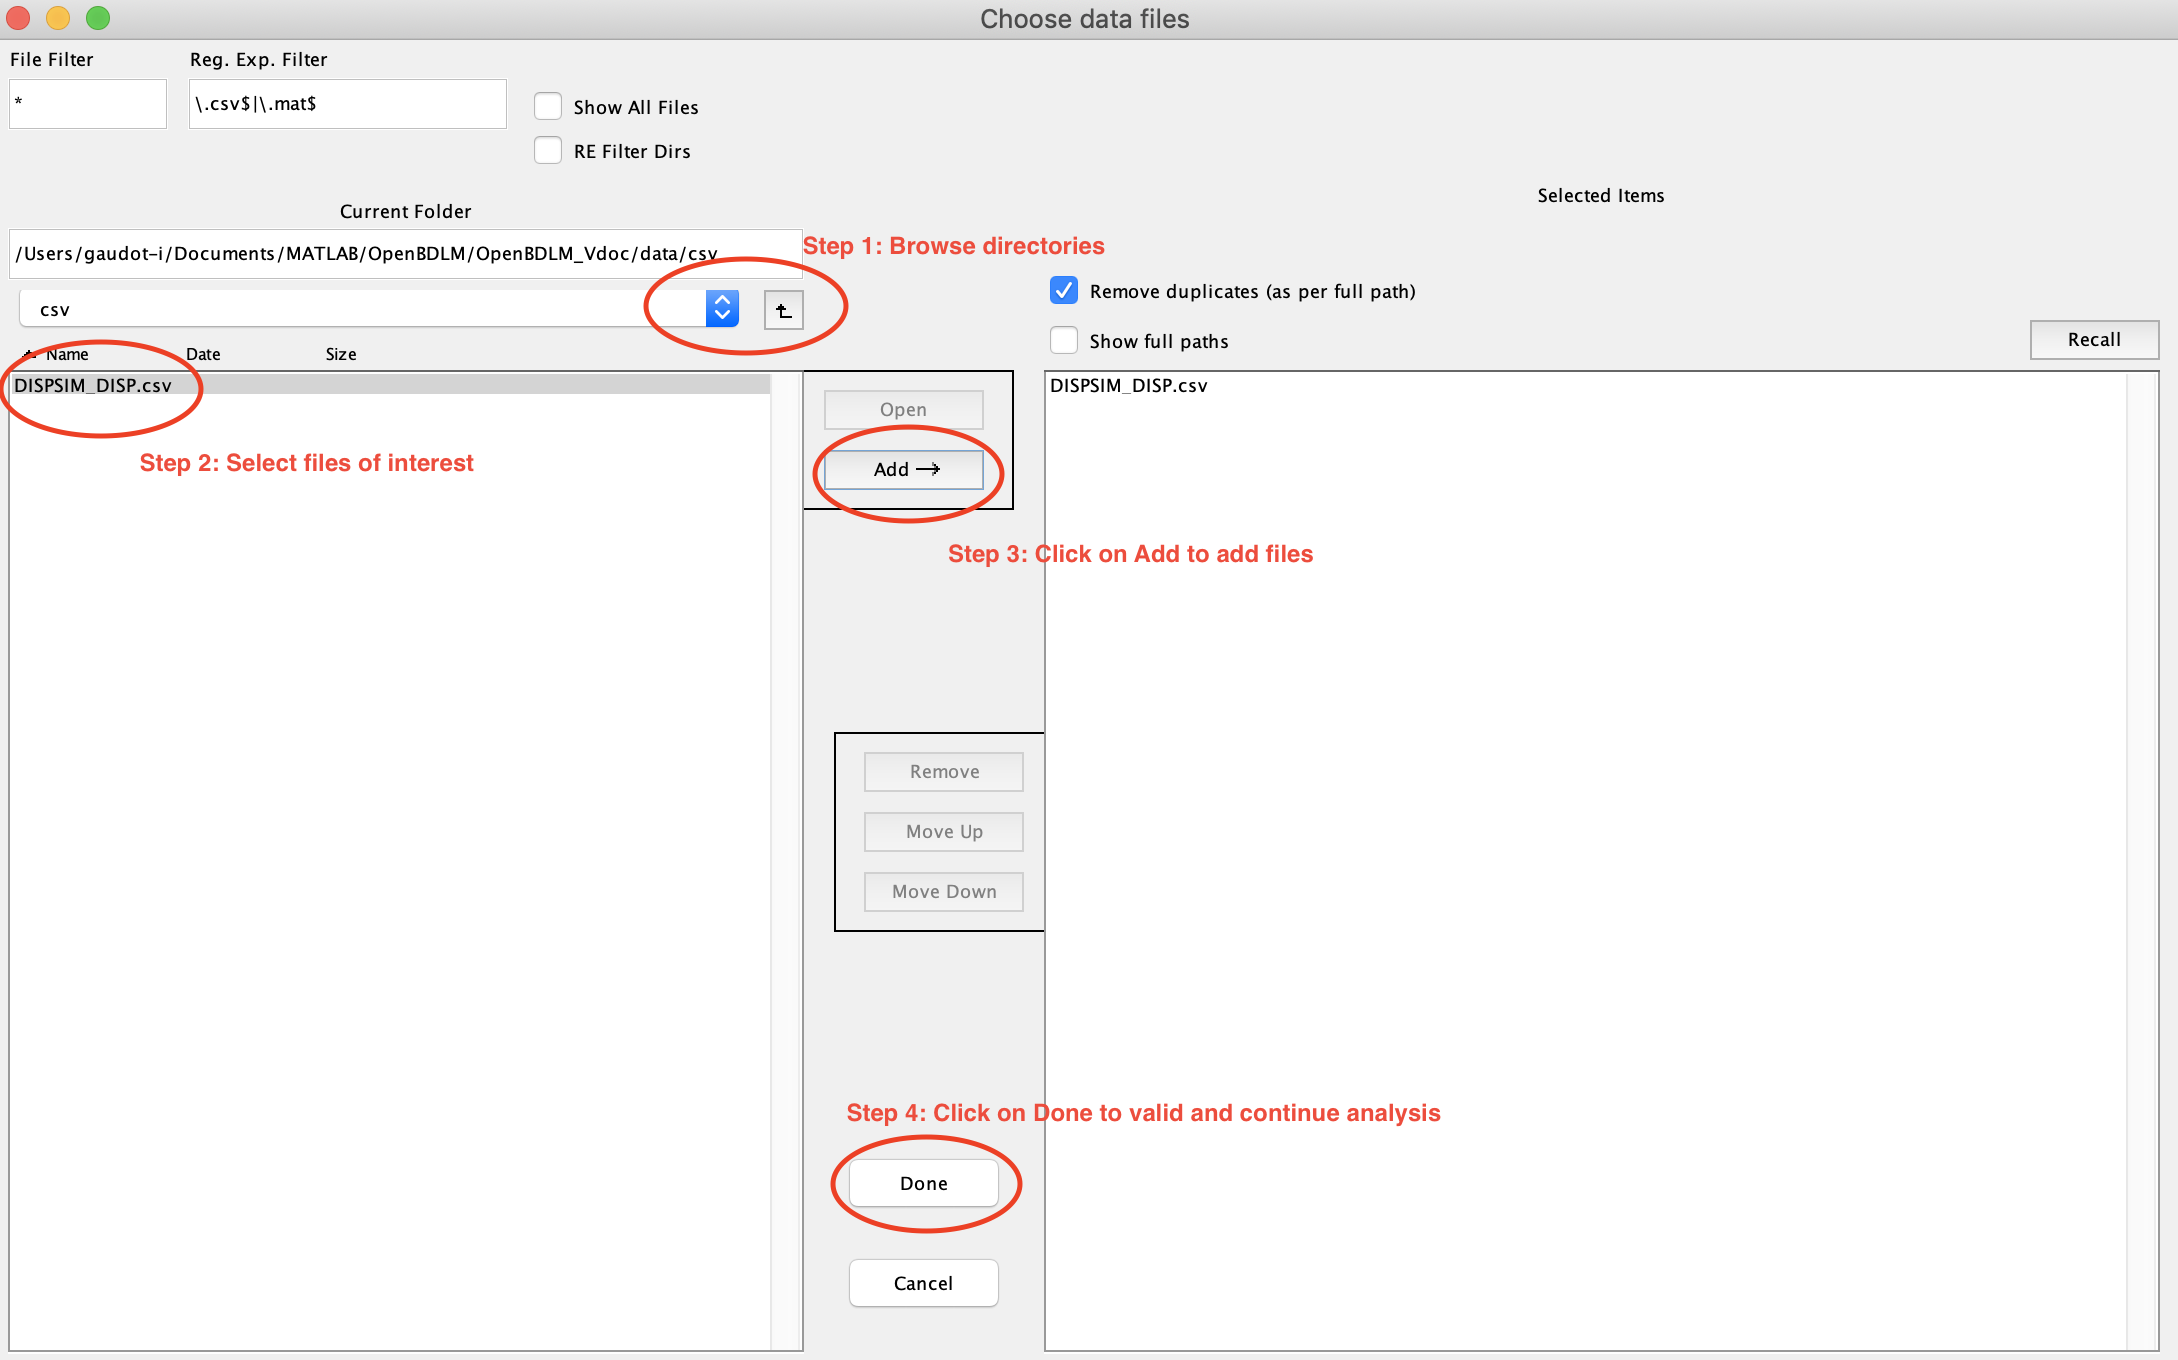
\includegraphics[width=0.9\linewidth]{./docfigs/Example_DISPSIM/dataloading_DISPSIM_uipickfiles_annoted.png}
\caption{Interactive data loading using the graphical user interface.}.
\label{fig:DataLoadingUIPickFileExample1}
\end{center}
\end{figure*}

 \begin{lstlisting}[ frame = single, basicstyle = \mlttfamily \small, caption = { \MATLAB{} command window output after selected data files.} from \MATLAB{} command line, label = LST:OpenBDLMDataAvailabilityExample1,  float =h!, linewidth=\linewidth, captionpos=b]
- Data available: 
 
     Time series number #      Reference name            Size                     	
     -----------------------------------------------------------------
     1                         DISP                      [19366x1]                	
     -----------------------------------------------------------------
\end{lstlisting}


\begin{figure*}[h!]
\centering
\begin{subfigure}{\linewidth}
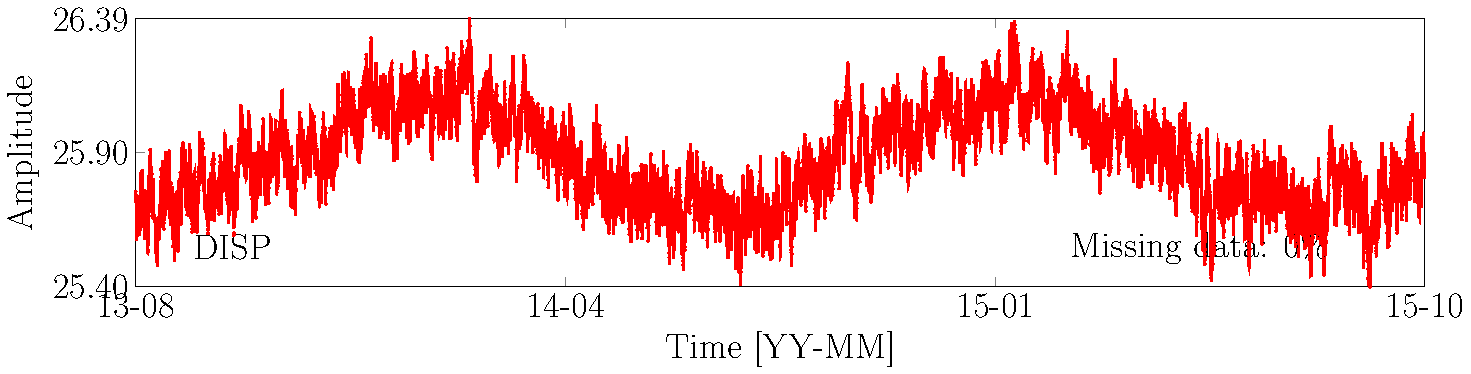
\includegraphics[width=0.9\linewidth]{./docfigs/Example_DISPSIM/raw/ALL_AMPLITUDES.pdf}
\caption{Amplitude}
\end{subfigure}
\begin{subfigure}{\linewidth}
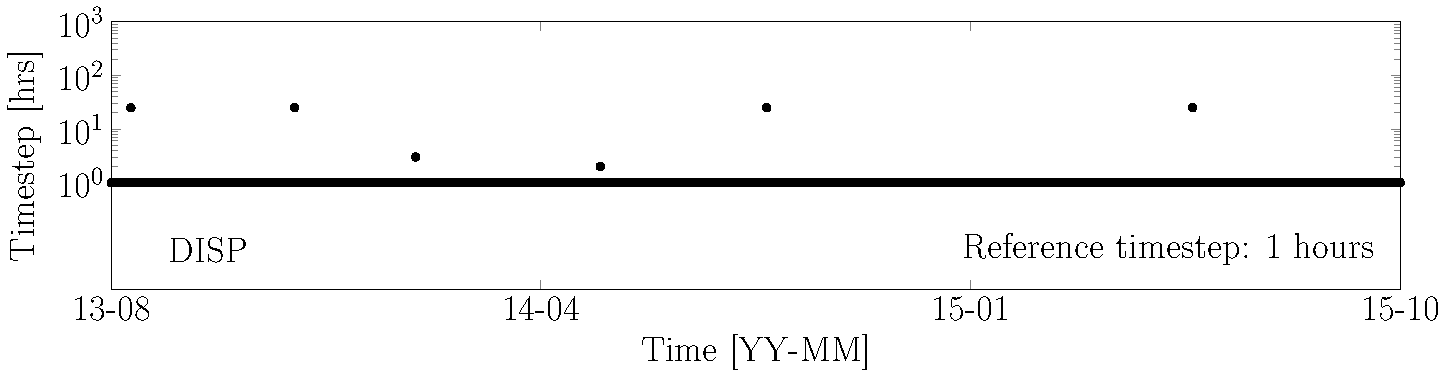
\includegraphics[width=0.9\linewidth]{./docfigs/Example_DISPSIM/raw/ALL_TIMESTEPS.pdf} 
\caption{Timestep}
\end{subfigure}
\begin{subfigure}{\linewidth}
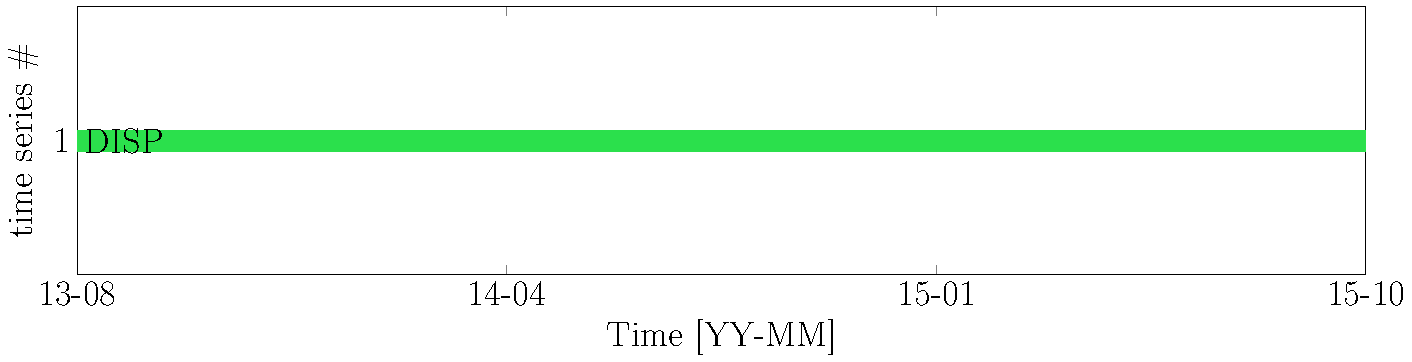
\includegraphics[width=0.9\linewidth]{./docfigs/Example_DISPSIM/raw/AVAILABILITY.pdf}
\caption{Availbility}
\end{subfigure}
\caption{Data used in Section~\ref{S:ExampleDisp}}.
\label{fig:DataSummary1}
\end{figure*}

\subsection{Step 3: edit and pre-process the data}

The next step of the analysis consists in editing or preprocessing the data.
The data editing and preprocessing menu as depicted in Listing~\ref{LST:Editing_menu} appear.
In this example, the objective is to use the data as such, so no editing or preprocessing is done.
Therefore, type \colorbox{light-gray}{\lstinline[basicstyle = \mlttfamily \small, backgroundcolor = \color{light-gray}]!7!} to save the data as such, and continue analysis.

\subsection{Step 4: configure the model}

The next step is to configure the model.
First, the program requests the number of model class.
In this exemple, the time series data looks stationary and we are not interested in anomaly detection, so type type \colorbox{light-gray}{\lstinline[basicstyle = \mlttfamily \small, backgroundcolor = \color{light-gray}]!1!}.
Secondly, OpenBDLM asks for the type of block component. 
Type \colorbox{light-gray}{\lstinline[basicstyle = \mlttfamily \small, backgroundcolor = \color{light-gray}]![11 31 31 41]!} to define a model with a local level, a yearly periodic component, a daily periodic component and an autoregressive component.
The  output on \MATLAB{} command window during interactive model configuration is presented in Listing~\ref{LST:OpenBDLMModelConfigureExample1}.
Type $\dlsh$ to valid.
The model is then built, a {\lstinline[basicstyle = \mlttfamily \small, backgroundcolor = \color{light-gray}]!DATA_DISP.mat!} binary data file, a {\lstinline[basicstyle = \mlttfamily \small, backgroundcolor = \color{light-gray}]!CFG_DISP.m!} configuration file, as well as a {\lstinline[basicstyle = \mlttfamily \small, backgroundcolor = \color{light-gray}]!PROJ_DISP.mat!} project file are created.
The OpenBLDM main menu must appear on the \MATLAB{} command window (see Listing~\ref{LST:OpenBDLMMainMenu}).
Type \colorbox{light-gray}{\lstinline[basicstyle = \mlttfamily \small, backgroundcolor = \color{light-gray}]!Q!} to save and quit.

 \begin{lstlisting}[ frame = single, basicstyle = \mlttfamily \small, caption = { \MATLAB{} command window output during interactive model configuration.}, label = LST:OpenBDLMModelConfigureExample1,  float =h, linewidth=\linewidth, captionpos=b]
- How many model classes do you want for each time-series? 
     choice >> 1
     
     --------------------------------------------------------
     BDLM Component reference numbers
     --------------------------------------------------------
     11: Local level 
     12: Local trend 
     13: Local acceleration 
     21: Local level compatible with local trend 
     22: Local level compatible with local acceleration 
     23: Local trend compatible with local acceleration 
     31: Periodic 
     41: Autoregressive process (AR(1)) 
     51: Kernel regression 
     61: Level Intervention 
     --------------------------------------------------------

- Identify components for time series #1; e.g. [11 31 41]
     choice >> [11 31 31 41]

     Building model...
     Saving project...
     Project saved in saved_projects/PROJ_DISP.mat. 
     Printing configuration file...
     Saving data...

     Database saved in data/mat/DATA_DISP.mat 
     Configuration file saved in config_files/CFG_DISP.m. 

\end{lstlisting}


\subsection{Step 5: open the configuration file}

After the data loading and the model configuration, a configuration file named \lstinline[basicstyle = \mlttfamily \small, backgroundcolor = \color{light-gray}]!CFG_DISP.csv! is automatically created and saved in ``config\_files'' folder.
Open the configuration file from \MATLAB{} command line by typing  \colorbox{light-gray}{\lstinline[basicstyle = \mlttfamily \small, backgroundcolor = \color{light-gray}]!edit CFG_DISP.m!}.
The first part of this configuration file as it should appear on the \MATLAB{} editor is shown in Listing~\ref{LST:CFGFileExample1}.
The Model parameters section of the configuration file shows that the model totalizes 8 model parameters, that is 
\begin{gather*}
\bm\theta=\{\sigma_{w}^{LL}, p^{\text{PD1}}, \sigma_{w}^{\text{PD1}} , p^{\text{PD2}}, \sigma_{w}^{\text{PD2}}, \phi^{AR}, \sigma_{w}^{AR}, \sigma_{v}\}.
\end{gather*}
%The default value of the model parameters are assigned   using heuristic knowledge or computed from the data using statistics on the data.
The default model parameters values are 
\begin{gather*}
\bm\theta^{\text{default}}=\{0, 365.2422, 0, 1, 0, 0.75, 0.0174, 0.0087002 \}.
\end{gather*}
%In the same manner, default value for the initial hidden states are assigned using heuristic knowledge or computed using statistics on the data.
The default  hidden states mean  and covariance values are 
\begin{align*}
\bm \mu^{\text{default}}_{0} & = [25.8 , 5  ,   	0     ,	5   ,  	0    , 	0     ]^{\intercal}, \text{and} \\
 \text{diag}(\bm\Sigma^{\text{default}}_{0}) & = [	0.121 	,0.121 ,	0.121 ,	0.121 ,	0.121 	, 0.0303     ], 
 \end{align*}
 respectively.

%\subsection{Step 6: results using defaults model parameters and default initial hidden states}

%Note that, by default, OpenBDLM considers that the parameters $\sigma_{w}^{LL}$, $P1$, $\sigma_{w}^{P1}$ , $P2$, $\sigma_{w}^{P2}$ are known.


% \lstinline[basicstyle = \mlttfamily \small ]!model.param_properties! 

\begin{lstlisting}[linewidth=\linewidth, style=Matlab-editor,  basicstyle = \mlttfamily \scriptsize, backgroundcolor = \color{matlab-yellow}, caption = {Example of a configuration file}, label=LST:CFGFileExample1, ,captionpos=b, float=h!]
%                    OpenBDLM configuration file                          
%          Autogenerated by OpenBDLM on 22-Nov-2018 17:18:09              
%
%% A - Project name
misc.ProjectName='DISP';

%% B - Data
dat=load('DATA_DISP.mat'); 
data.values=dat.values;
data.timestamps=dat.timestamps;
data.labels={'DISP'};

%% C - Model structure 
% Components reference numbers
% 11: Local level
% 12: Local trend
% 13: Local acceleration
% 21: Local level compatible with local trend
% 22: Local level compatible with local acceleration
% 23: Local trend compatible with local acceleration
% 31: Periodic
% 41: Autoregressive
% 51: Kernel regression
% 61: Level Intervention

% Model components
% Model 1
model.components.block{1}={[11 31 31 41] };

% Model component constrains | Take the same  parameter as model class #1
 
% Model inter-components dependence | {[components form dataset_i depends on components from  dataset_j]_i,[...]}
model.components.ic={[ ] };
%
%% D - Model parameters 
model.param_properties={
     % #1       #2       #3    #4    #5         #6       #7     #8     #9    #10
     % Param name Block name  Model Obs Bound Prior Mean Std Values Ref
     '\sigma_w', 'LL',  '1',   '1', [NaN  NaN],    'N/A',  NaN, NaN,  0,          1 %#1   
     'p',        'PD1', '1',   '1', [NaN  NaN],    'N/A',  NaN, NaN, 365.24,      2 %#2   
     '\sigma_w', 'PD1', '1',   '1', [NaN  NaN],    'N/A',  NaN, NaN,   0,         3 %#3   
     'p',        'PD2', '1',   '1', [NaN  NaN],    'N/A',  NaN, NaN,   1,         4 %#4   
     '\sigma_w', 'PD2', '1',   '1', [NaN  NaN],    'N/A',  NaN, NaN,   0,         5 %#5   
     '\phi',     'AR',  '1',   '1', [0  1],        'N/A',  NaN, NaN,   0.75,      6 %#6   
     '\sigma_w', 'AR',  '1',   '1', [0  Inf],      'N/A',  NaN, NaN,   0.0174,    7 %#7   
     '\sigma_v', '',    '1',   '1', [0  Inf],      'N/A',  NaN, NaN,   0.0087002, 8 %#8   
};

%% E - Initial states values 
% Initial hidden states mean for model 1:
model.initX{ 1 }=[	25.8  	5     	0     	5     	0     	0     ]';

% Initial hidden states variance for model 1: 
model.initV{ 1 }=diag([ 	0.121 	0.121 	0.121 	0.121 	0.121 	0.0303 ]);

% Initial probability for model 1
model.initS{1}=[1     ];

\end{lstlisting}

\subsection{Step 6: estimate the hidden states}

Type \colorbox{light-gray}{\lstinline[basicstyle = \mlttfamily \small, backgroundcolor = \color{light-gray}]!OpenBDLM_main('CFG_DISP.m');!} in the \MATLAB{} command line.
Once, the main menu appears, type  \colorbox{light-gray}{\lstinline[basicstyle = \mlttfamily \small, backgroundcolor = \color{light-gray}]!3!}, then \colorbox{light-gray}{\lstinline[basicstyle = \mlttfamily \small, backgroundcolor = \color{light-gray}]!1!} to estimate the filtered hidden states using the default model parameters and default initial hidden states values.
The value of the log-likelihood is $38627$, and the estimated hidden states are presented in Figure~\ref{fig:DISPSIMDefaultDefaultExample1}.

\begin{figure*}[h!]
\centering
\begin{subfigure}{\linewidth}
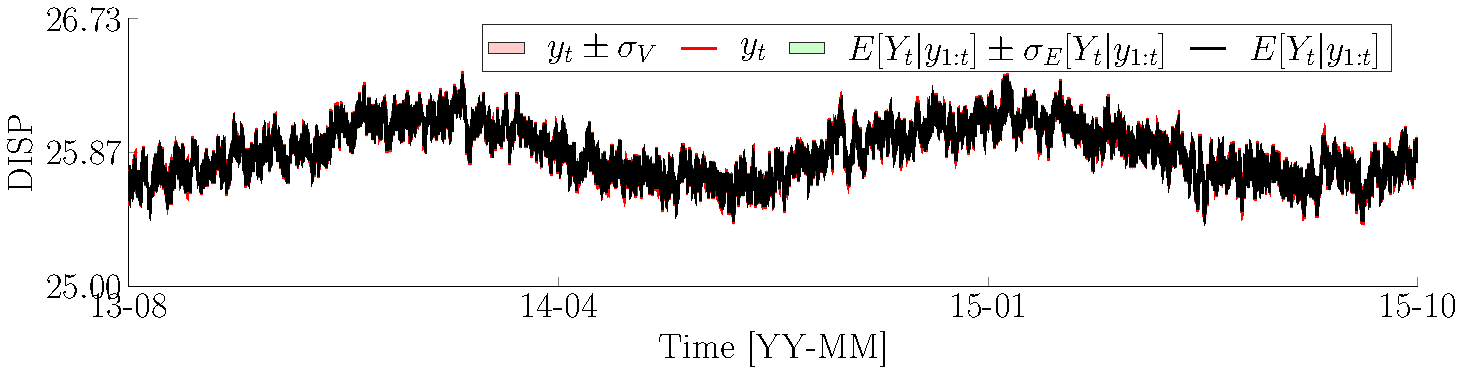
\includegraphics[width=0.9\linewidth]{./docfigs/Example_DISPSIM/default/DISP_ObservedPredicted.pdf} 
\caption{Observed and estimated displacement data}
\end{subfigure}
\begin{subfigure}{\linewidth}
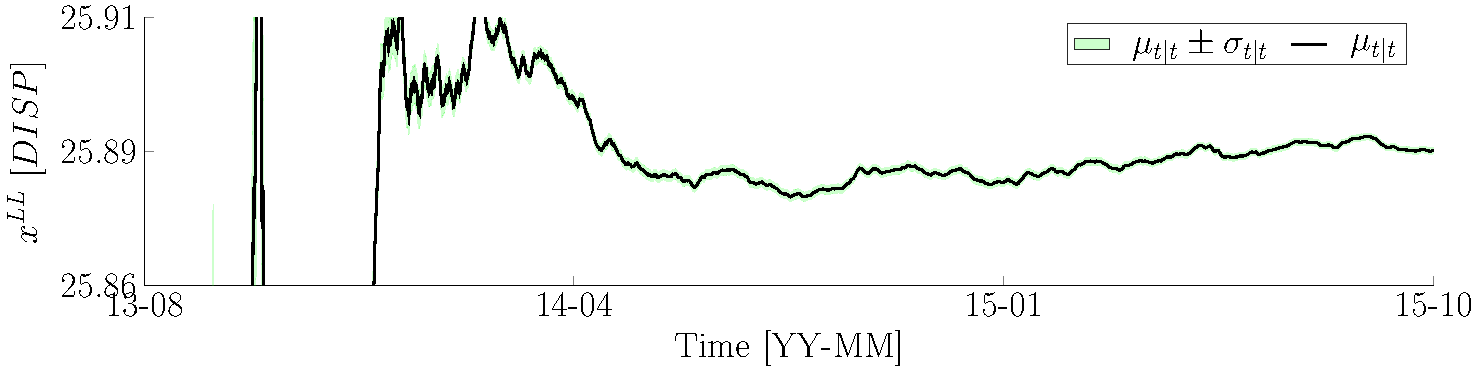
\includegraphics[width=0.9\linewidth]{./docfigs/Example_DISPSIM/default/DISP_LL_1.pdf}
\caption{Estimated displacement local level component}.
\end{subfigure}
\begin{subfigure}{\linewidth}
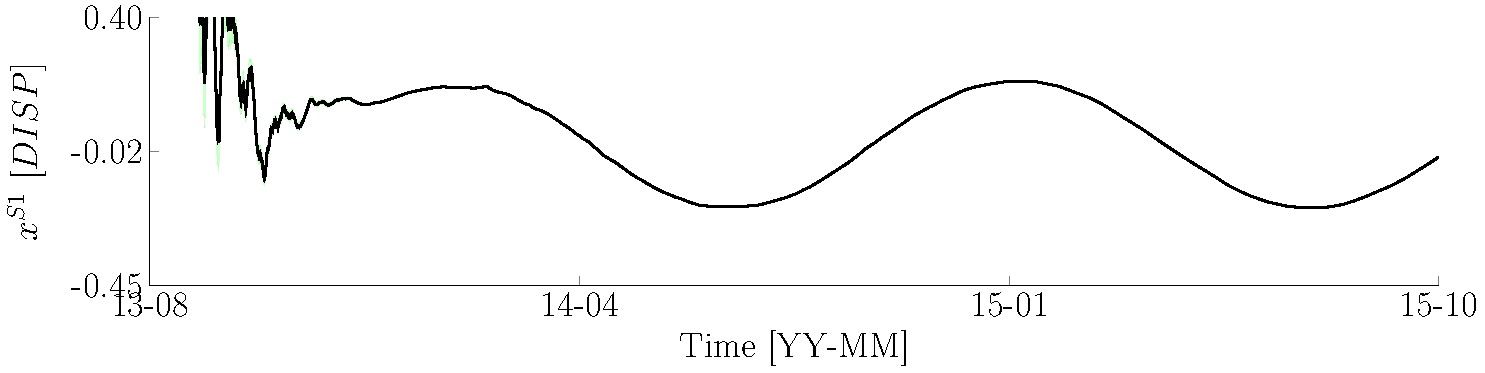
\includegraphics[width=0.9\linewidth]{./docfigs/Example_DISPSIM/default/DISP_S1_2.pdf}
\caption{Estimated displacement yearly periodic component}
\end{subfigure}
\begin{subfigure}{\linewidth}
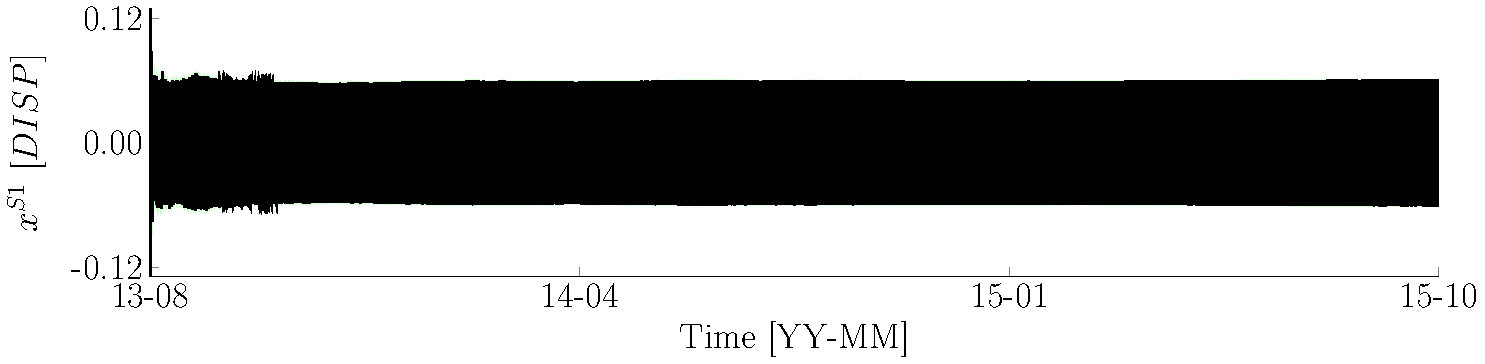
\includegraphics[width=0.9\linewidth]{./docfigs/Example_DISPSIM/default/DISP_S1_4.pdf}
\caption{Estimated displacement daily periodic component}
\end{subfigure}
\begin{subfigure}{\linewidth}
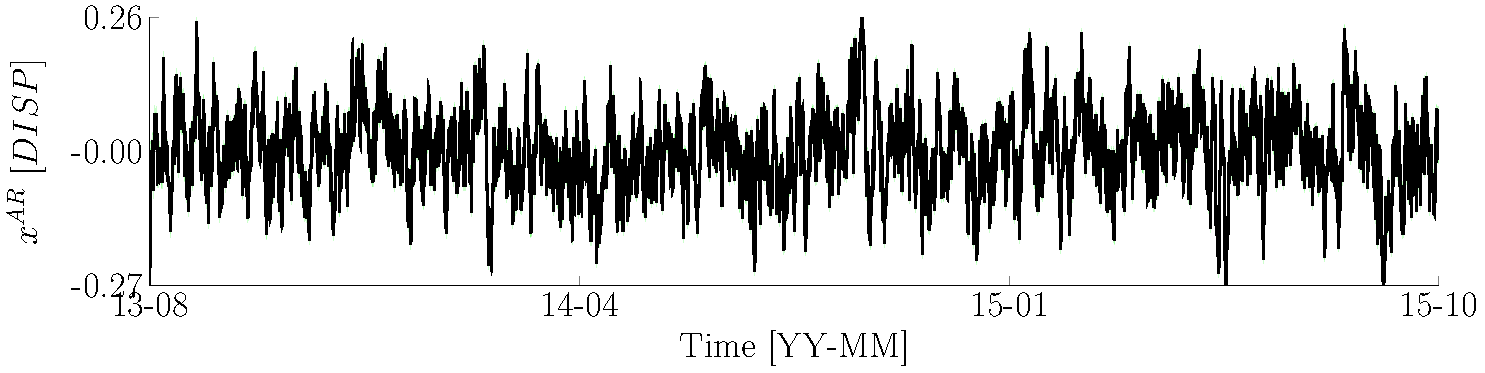
\includegraphics[width=0.9\linewidth]{./docfigs/Example_DISPSIM/default/DISP_AR_6.pdf} 
\caption{Estimated displacement autoregressive component}
\end{subfigure}
\caption{Estimated results using OpenBDLM defaults model parameters and default initial hidden states. The hidden states are estimated from the data presented in Figure~\ref{fig:DataSummary1}a. The solid line and shaded area represent the mean and standard deviation of the estimated hidden states, respectively.}
\label{fig:DISPSIMDefaultDefaultExample1}
\end{figure*}

\subsection{Step 7: estimate the model parameters from the data}

Type \colorbox{light-gray}{\lstinline[basicstyle = \mlttfamily \small, backgroundcolor = \color{light-gray}]!OpenBDLM_main('CFG_DISP.m');!} in the \MATLAB{} command line.
Once, the main menu appears, type  \colorbox{light-gray}{\lstinline[basicstyle = \mlttfamily \small, backgroundcolor = \color{light-gray}]!1!}, then \colorbox{light-gray}{\lstinline[basicstyle = \mlttfamily \small, backgroundcolor = \color{light-gray}]!1!} to estimate the model parameters using Newton-Raphson (type  \colorbox{light-gray}{\lstinline[basicstyle = \mlttfamily \small, backgroundcolor = \color{light-gray}]!1!} to use the Stochastic Gradient instead).
The model parameters learning procedure starts, and messages are printed on \MATLAB{} command window to monitor the convergence through iterations (see Listing~\ref{LST:OpenBLDMModelParameterLearning}).
Note that, by default, OpenBDLM considers that the parameters $\sigma_{w}^{LL}$, $PD1$, $\sigma_{w}^{PD1}$ , $PD2$, $\sigma_{w}^{PD2}$ are known.
Therefore, there are three model parameters to be learned from the data in this example.
The estimation of the model parameters may take several hours.
Once the algorithm converged, the optimized model parameters values should be close to \footnote{Note that it is possible to get slightly different value of parameters with the same performance.}
\begin{gather*}
\bm\theta^{\text{*}}=\{0, 365.2422, 0, 1, 0, 0.97, 0.0192, 7.4258\times10^{-7} \}.
\end{gather*}

\subsection{Step 8: estimate the hidden states using the optimized model parameters values}

Type \colorbox{light-gray}{\lstinline[basicstyle = \mlttfamily \small, backgroundcolor = \color{light-gray}]!OpenBDLM_main('CFG_DISP_optim.m');!} in the \MATLAB{} command line to load the configuration file  \lstinline[basicstyle = \mlttfamily \small, backgroundcolor = \color{light-gray}]!CFG_DISP_optim.m'!.
 \lstinline[basicstyle = \mlttfamily \small, backgroundcolor = \color{light-gray}]!CFG_DISP_optim.m'! contains optimized model parameters previously estimated using the Newton-Raphson algorithm.
Once the main menu appears, type  \colorbox{light-gray}{\lstinline[basicstyle = \mlttfamily \small, backgroundcolor = \color{light-gray}]!3!}, then \colorbox{light-gray}{\lstinline[basicstyle = \mlttfamily \small, backgroundcolor = \color{light-gray}]!1!} to estimate the filtered hidden states using the optimized model parameters and default initial hidden states values.
The value of the log-likelihood is now $48819$.
The estimated hidden states are presented in Figure~\ref{fig:DISPSIMOptimizedDefaultExample1}.

\begin{figure*}[h!]
\begin{center}
\begin{subfigure}{\linewidth}
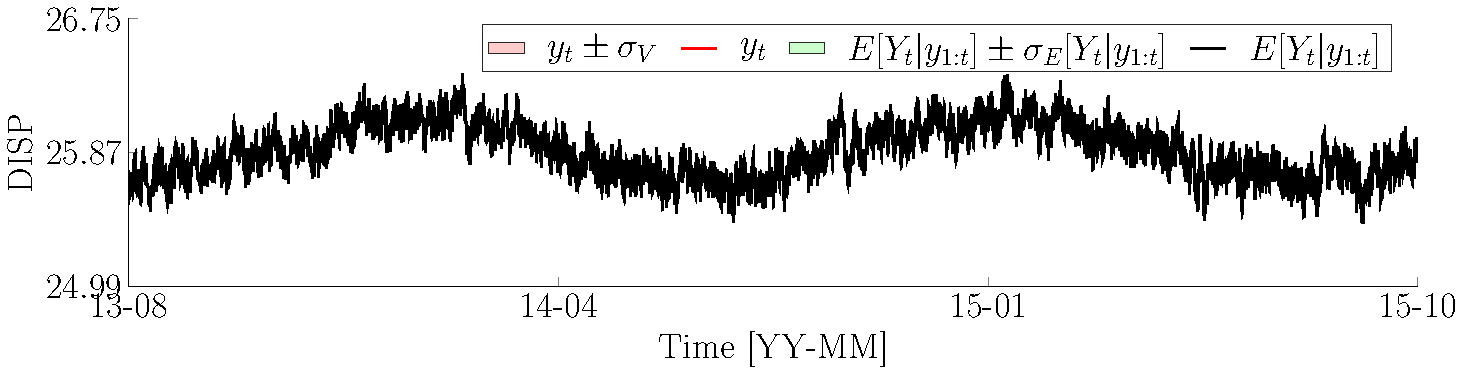
\includegraphics[width=0.9\linewidth]{./docfigs/Example_DISPSIM/optim_param_default_initialhiddenstate/DISP_ObservedPredicted.pdf}
\caption{Observed and estimated displacement data}
\end{subfigure}
\begin{subfigure}{\linewidth}
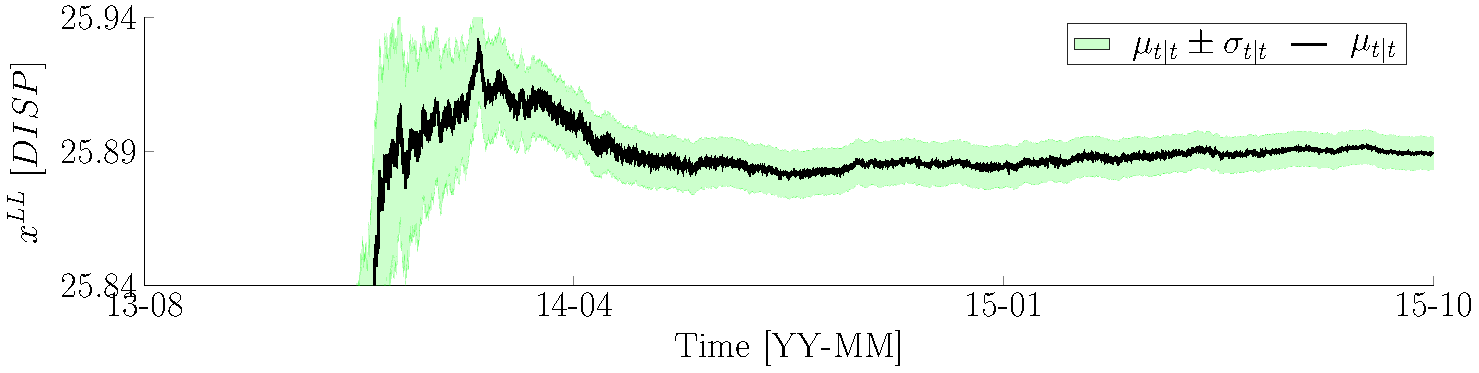
\includegraphics[width=0.9\linewidth]{./docfigs/Example_DISPSIM/optim_param_default_initialhiddenstate/DISP_LL_1.pdf}
\caption{Estimated displacement local level.}
\end{subfigure}
\begin{subfigure}{\linewidth}
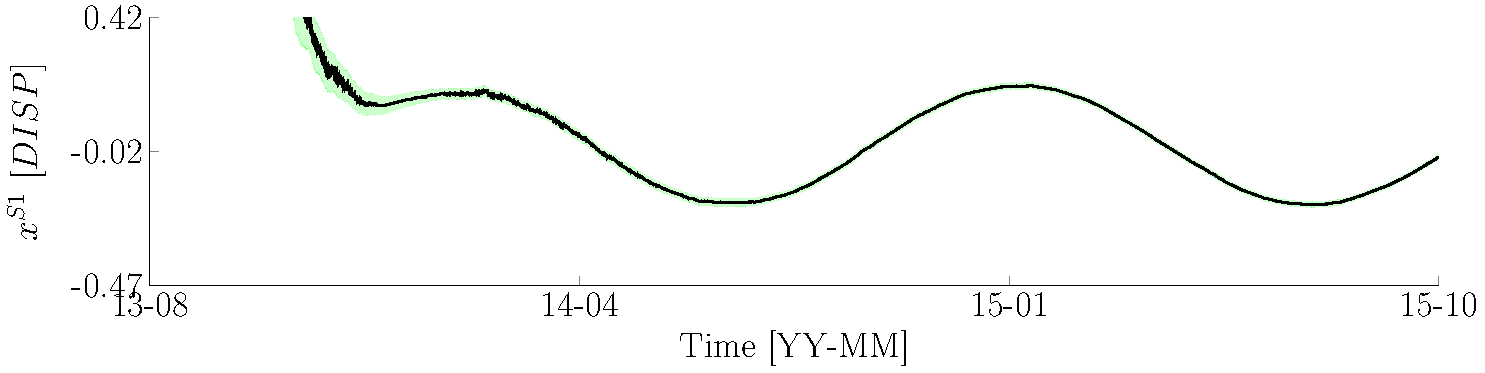
\includegraphics[width=0.9\linewidth]{./docfigs/Example_DISPSIM/optim_param_default_initialhiddenstate/DISP_S1_2.pdf}
\caption{Estimated displacement yearly periodic component (first hidden state)}
\end{subfigure}
\begin{subfigure}{\linewidth}
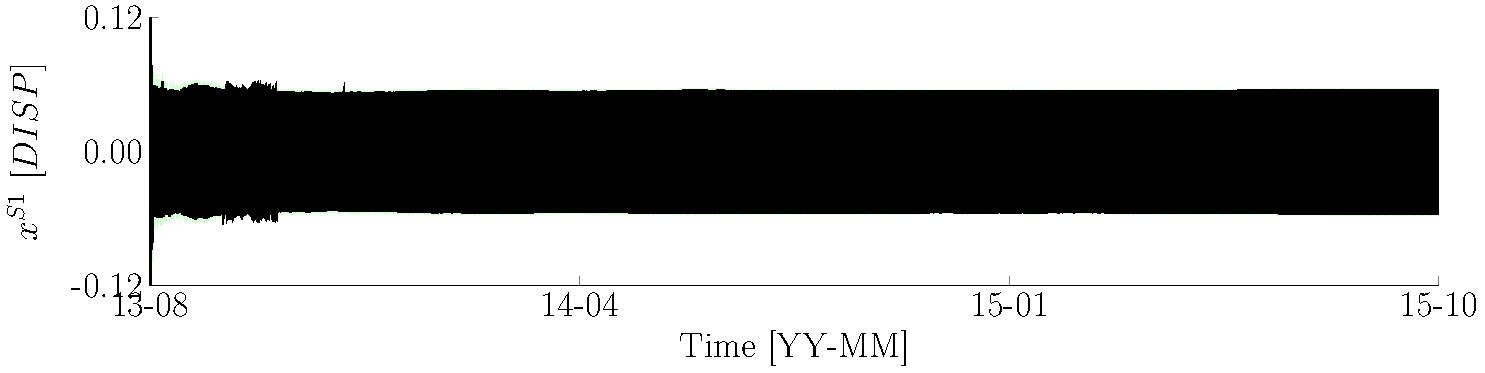
\includegraphics[width=0.9\linewidth]{./docfigs/Example_DISPSIM/optim_param_default_initialhiddenstate/DISP_S1_4.pdf} 
\caption{Estimated displacement daily periodic component (first hidden state)}
\end{subfigure}
\begin{subfigure}{\linewidth}
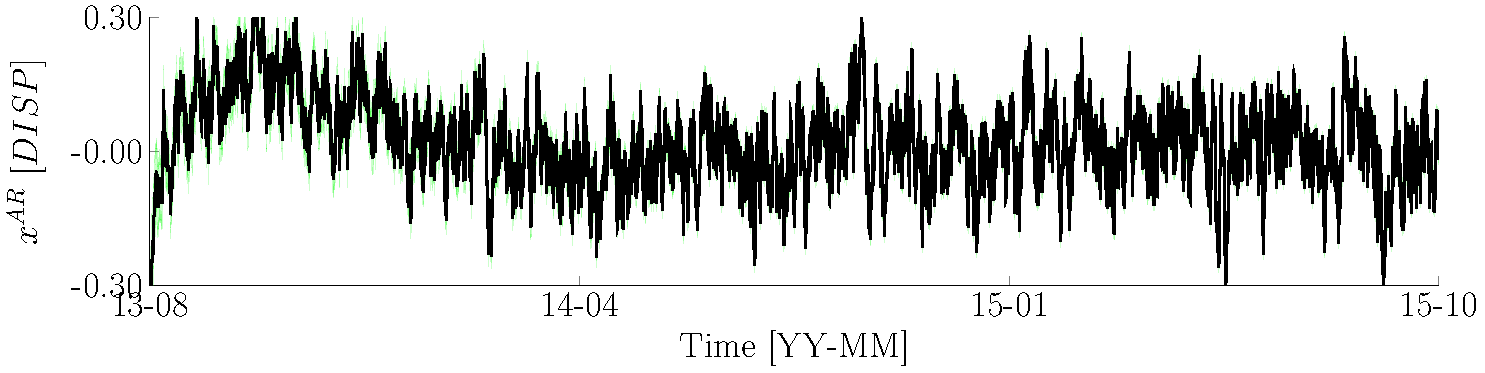
\includegraphics[width=0.9\linewidth]{./docfigs/Example_DISPSIM/optim_param_default_initialhiddenstate/DISP_AR_6.pdf} 
\caption{Estimated displacement autoregressive component}
\end{subfigure}
\caption{Estimated results using OpenBDLM optimized model parameters and default initial hidden states. The hidden states are estimated from the data presented in Figure~\ref{fig:DataSummary1}a. The solid line and shaded area represent the mean and standard deviation of the estimated hidden states, respectively.}
\label{fig:DISPSIMOptimizedDefaultExample1}
\end{center}
\end{figure*}

\subsection{Step 9: estimate the initial hidden states}

Type \colorbox{light-gray}{\lstinline[basicstyle = \mlttfamily \small, backgroundcolor = \color{light-gray}]!OpenBDLM_main('CFG_DISP_optim.m');!} in the \MATLAB{} command line.
Then, type  \colorbox{light-gray}{\lstinline[basicstyle = \mlttfamily \small, backgroundcolor = \color{light-gray}]!2!}, to optimize the initial hidden states value.
The estimated initial hidden states mean and covariance values are 
\begin{align*}
\bm \mu^{*}_{0} & = [	25.9  ,	-0.204,	-0.00288 ,	0.0341,	0.0521	, -0.0436  ]^{\intercal}, \text{and} \\
 \text{diag}(\bm\Sigma^{*}_{0}) & = [	3.74\times10^{-5} ,	6.87\times10^{-5}	, 7\times10^{-5} ,	5.73\times10^{-7} ,	5.73\times10^{-7} ,	0.000493    ], 
 \end{align*}
 respectively.
Once it is done, type  \colorbox{light-gray}{\lstinline[basicstyle = \mlttfamily \small, backgroundcolor = \color{light-gray}]!2!}, and then  \colorbox{light-gray}{\lstinline[basicstyle = \mlttfamily \small, backgroundcolor = \color{light-gray}]!1!} to compute the filtered hidden states using the optimized model parameters and optimized initial hidden states.
The value of the log-likelihood is $49056$.
The estimated hidden states are presented in Figure~\ref{fig:DISPSIMOptimizedOptimizedExample1}.


\begin{figure*}[h!]
\begin{center}
\begin{subfigure}{\linewidth}
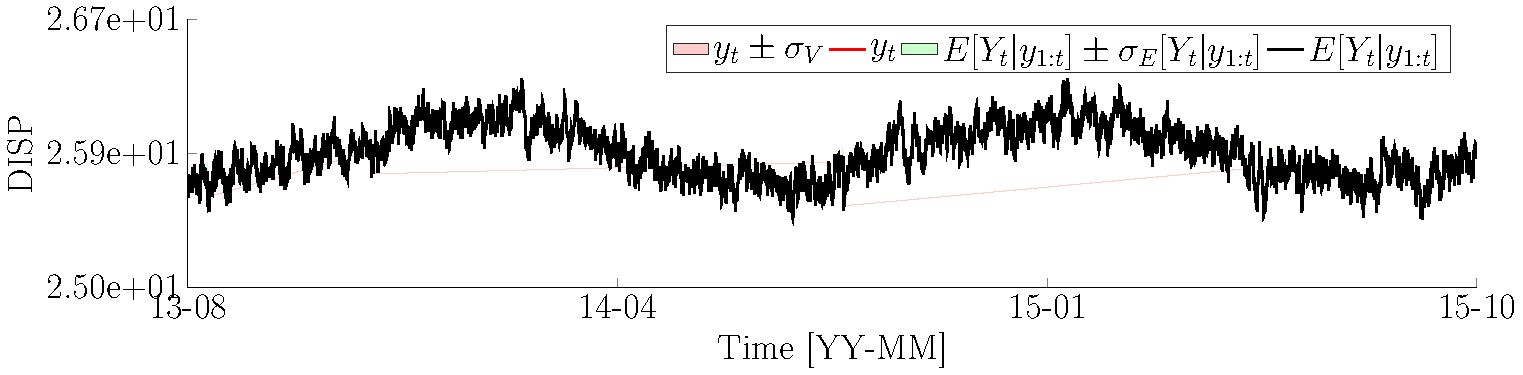
\includegraphics[width=0.9\linewidth]{./docfigs/Example_DISPSIM/optim_param_optim_initialhiddenstate/DISP_ObservedPredicted.pdf} 
\caption{Observed and estimated displacement data}
\end{subfigure}
\begin{subfigure}{\linewidth}
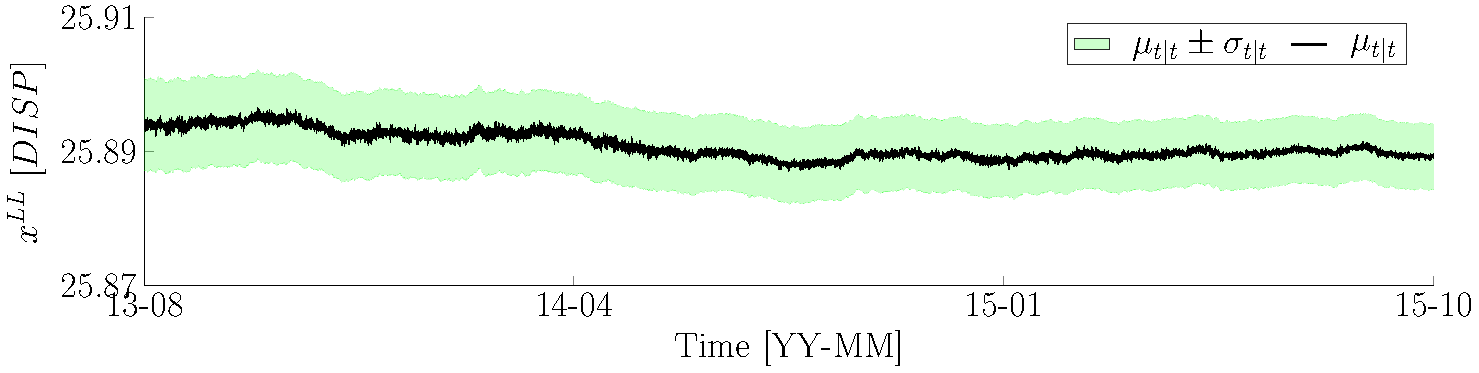
\includegraphics[width=0.9\linewidth]{./docfigs/Example_DISPSIM/optim_param_optim_initialhiddenstate/DISP_LL_1.pdf}
\caption{Estimated displacement local level component.}
\end{subfigure}
\begin{subfigure}{\linewidth}
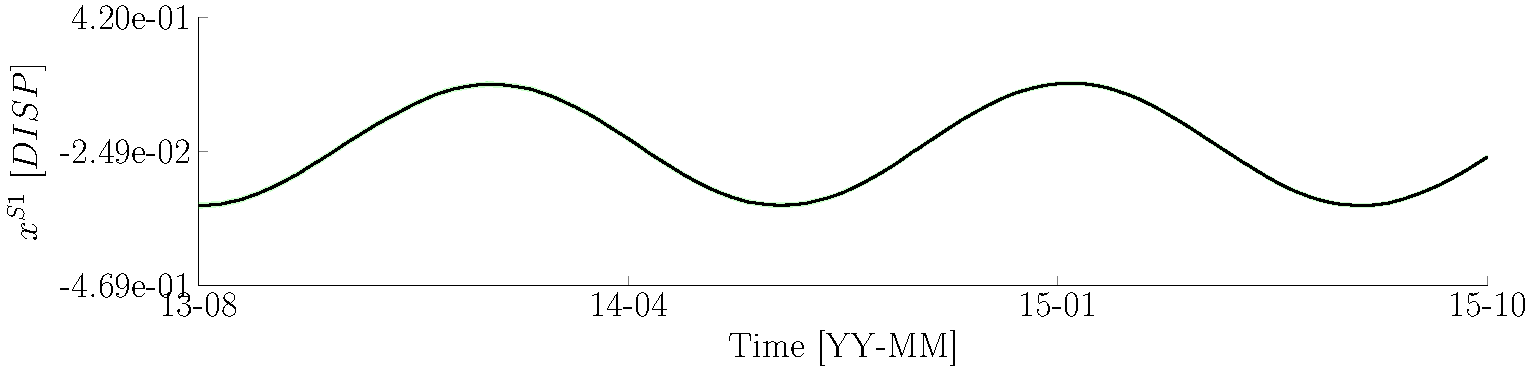
\includegraphics[width=0.9\linewidth]{./docfigs/Example_DISPSIM/optim_param_optim_initialhiddenstate/DISP_S1_2.pdf} 
\caption{Estimated displacement yearly periodic component (first hidden state)}
\end{subfigure}
\begin{subfigure}{\linewidth}
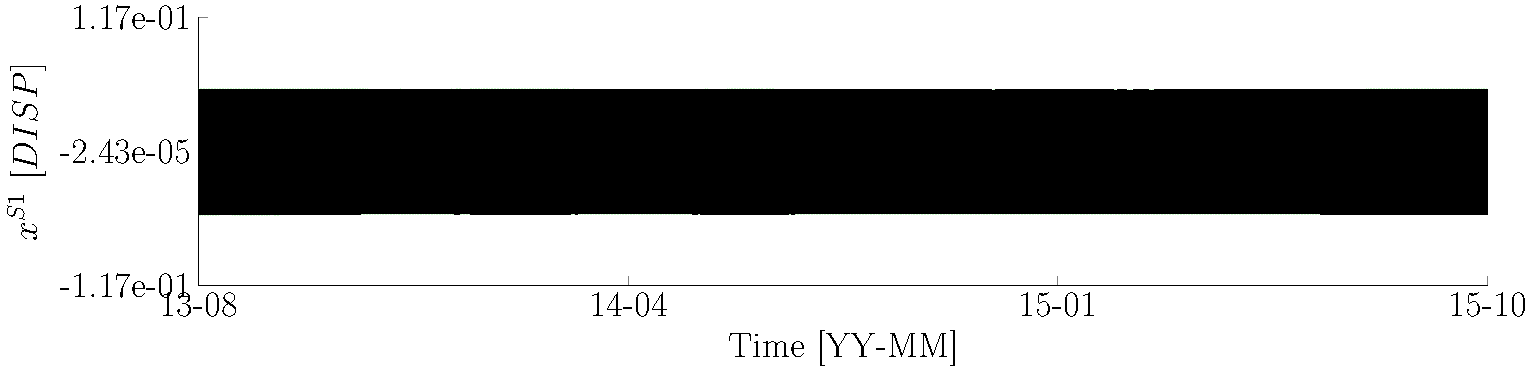
\includegraphics[width=0.9\linewidth]{./docfigs/Example_DISPSIM/optim_param_optim_initialhiddenstate/DISP_S1_4.pdf}
\caption{Estimated displacement daily periodic component (first hidden state)}
\end{subfigure}
\begin{subfigure}{\linewidth}
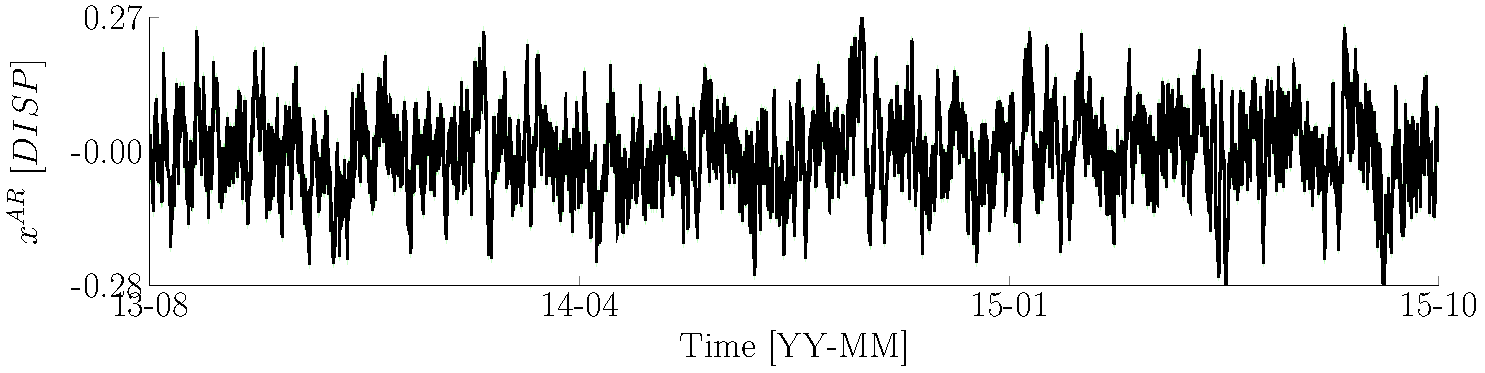
\includegraphics[width=0.9\linewidth]{./docfigs/Example_DISPSIM/optim_param_optim_initialhiddenstate/DISP_AR_6.pdf} 
\caption{Estimated displacement autoregressive component}
\end{subfigure}
\caption{Estimated results using OpenBDLM optimized model parameters and optimized initial hidden states. The hidden states are estimated from the data presented in Figure~\ref{fig:DataSummary1}a. The solid line and shaded area represent the mean and standard deviation of the estimated hidden states, respectively.}
\label{fig:DISPSIMOptimizedOptimizedExample1}
\end{center}
\end{figure*}